\maketitle

\begin{frame}
  \frametitle{HEP Software Foundation -- Community White Paper}
  \begin{columns}
    \begin{column}{.3\textwidth}
      
\includegraphics[width=\textwidth]{./hsf_logo_angled.png}
    \end{column}
    \begin{column}{.7\textwidth}
      \begin{itemize}
        \item Editing meeting on Friday
        \item Thanks to all contributors and commentators
          \begin{itemize}
            \item Comment deadline extended until 1st November
          \end{itemize}
      \end{itemize}
    \end{column}
  \end{columns}
\end{frame}

\begin{frame}
  \frametitle{Recordings online}
  \begin{columns}
    \begin{column}{.6\textwidth}
      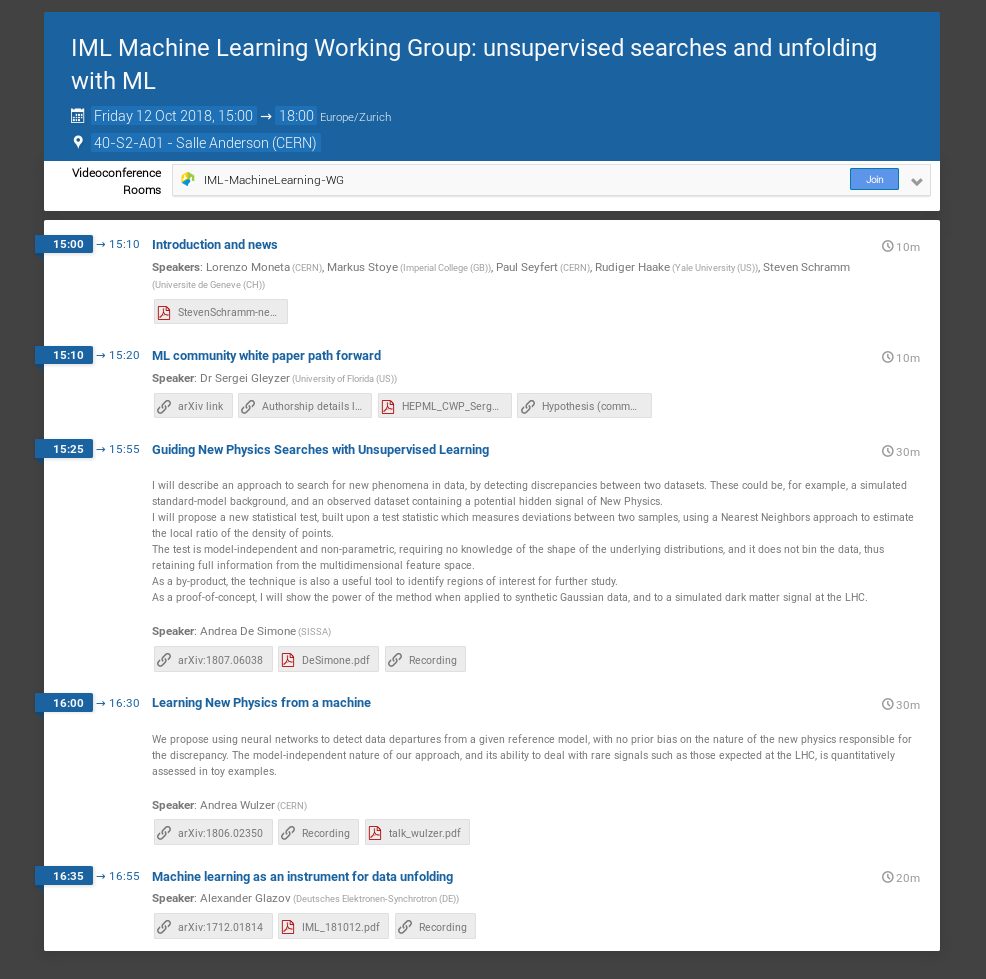
\includegraphics[width=.95\textwidth]{./rec.png}
    \end{column}
    \begin{column}{.4\textwidth}
      \begin{itemize}
        \item Instead of written minutes we now organise recordings for talks
        \item (with approval by the speaker, not automatically)
        \item e.g.\ last meeting's talks accessible on the indico agenda
        \item {\Large{Big thanks to the recording service}}
      \end{itemize}
    \end{column}
  \end{columns}
\end{frame}

\begin{frame}
  \frametitle{Upcoming events}
  \begin{description}
    \item[2018-10-31] \myhref{https://indico.cern.ch/event/760693/}{Data science seminar: Full Event Interpretation at Belle 2}
    \item[2018-11-30] \myhref{https://indico.cern.ch/event/762583/}{Next IML meeting (Filtration plant 222/R-001)}
      \newline open topic: anything ML related that you're working on that didn't fit topical meetings
  \end{description}
\end{frame}
\begin{frame}
  \frametitle{Upcoming conferences/workshops}
  \begin{description}
    \item[2018-11-14 -- 2018-11-16] \myhref{https://indico.cern.ch/event/745718/}{ML4Jets} abstract deadline tomorrow
      \newline ML as applied to jet physics
    \item[2019-01-22 -- 2019-01-25] \myhref{https://indico.cern.ch/event/735431/}{PHYSTAT-nu} abstract deadline tomorrow
      \newline statistics, including ML, for neutrino physics
    \item[2019-03-11 -- 2019-03-15] \myhref{https://indico.cern.ch/event/708041/}{ACAT} abstract deadline 2018-11-20
      \newline Empowering the Revolution: Bringing ML to HPC
    \item[2019-04-02 -- 2019-04-05] \myhref{https://indico.cern.ch/event/742793/}{Connecting the Dots} abstract deadline Sunday
      \newline track reconstruction, pattern recognition, and ML with tracks
  \end{description}
\end{frame}

\begin{frame}
  \frametitle{Today's meeting}
  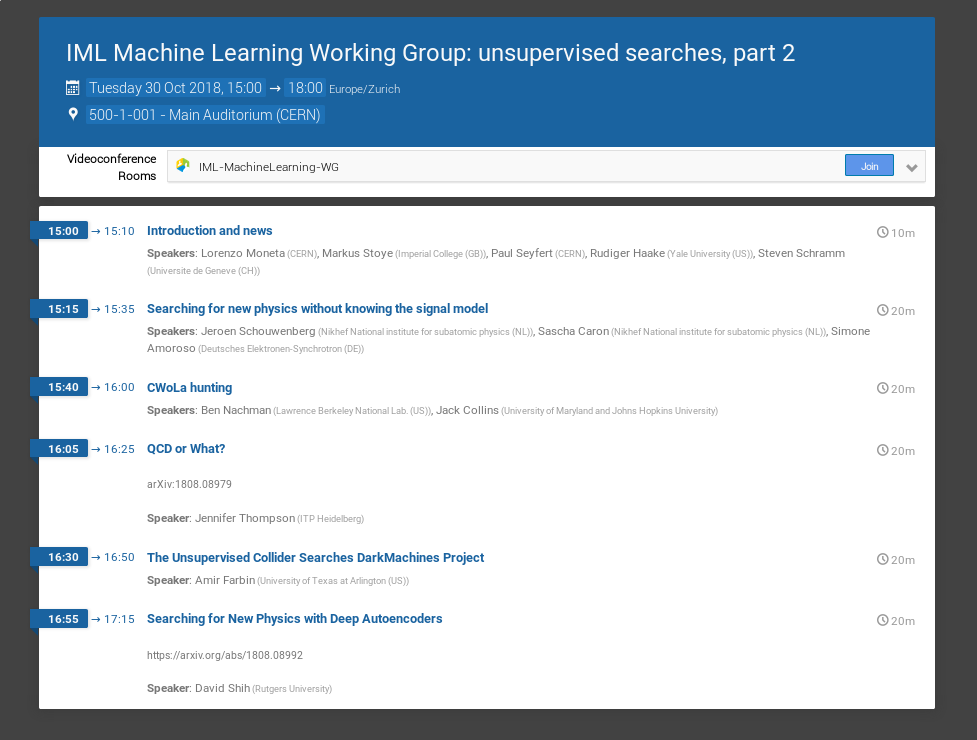
\includegraphics[width=.9\textwidth]{./agenda.png}
\end{frame}

\setbeamertemplate{background canvas}{%
  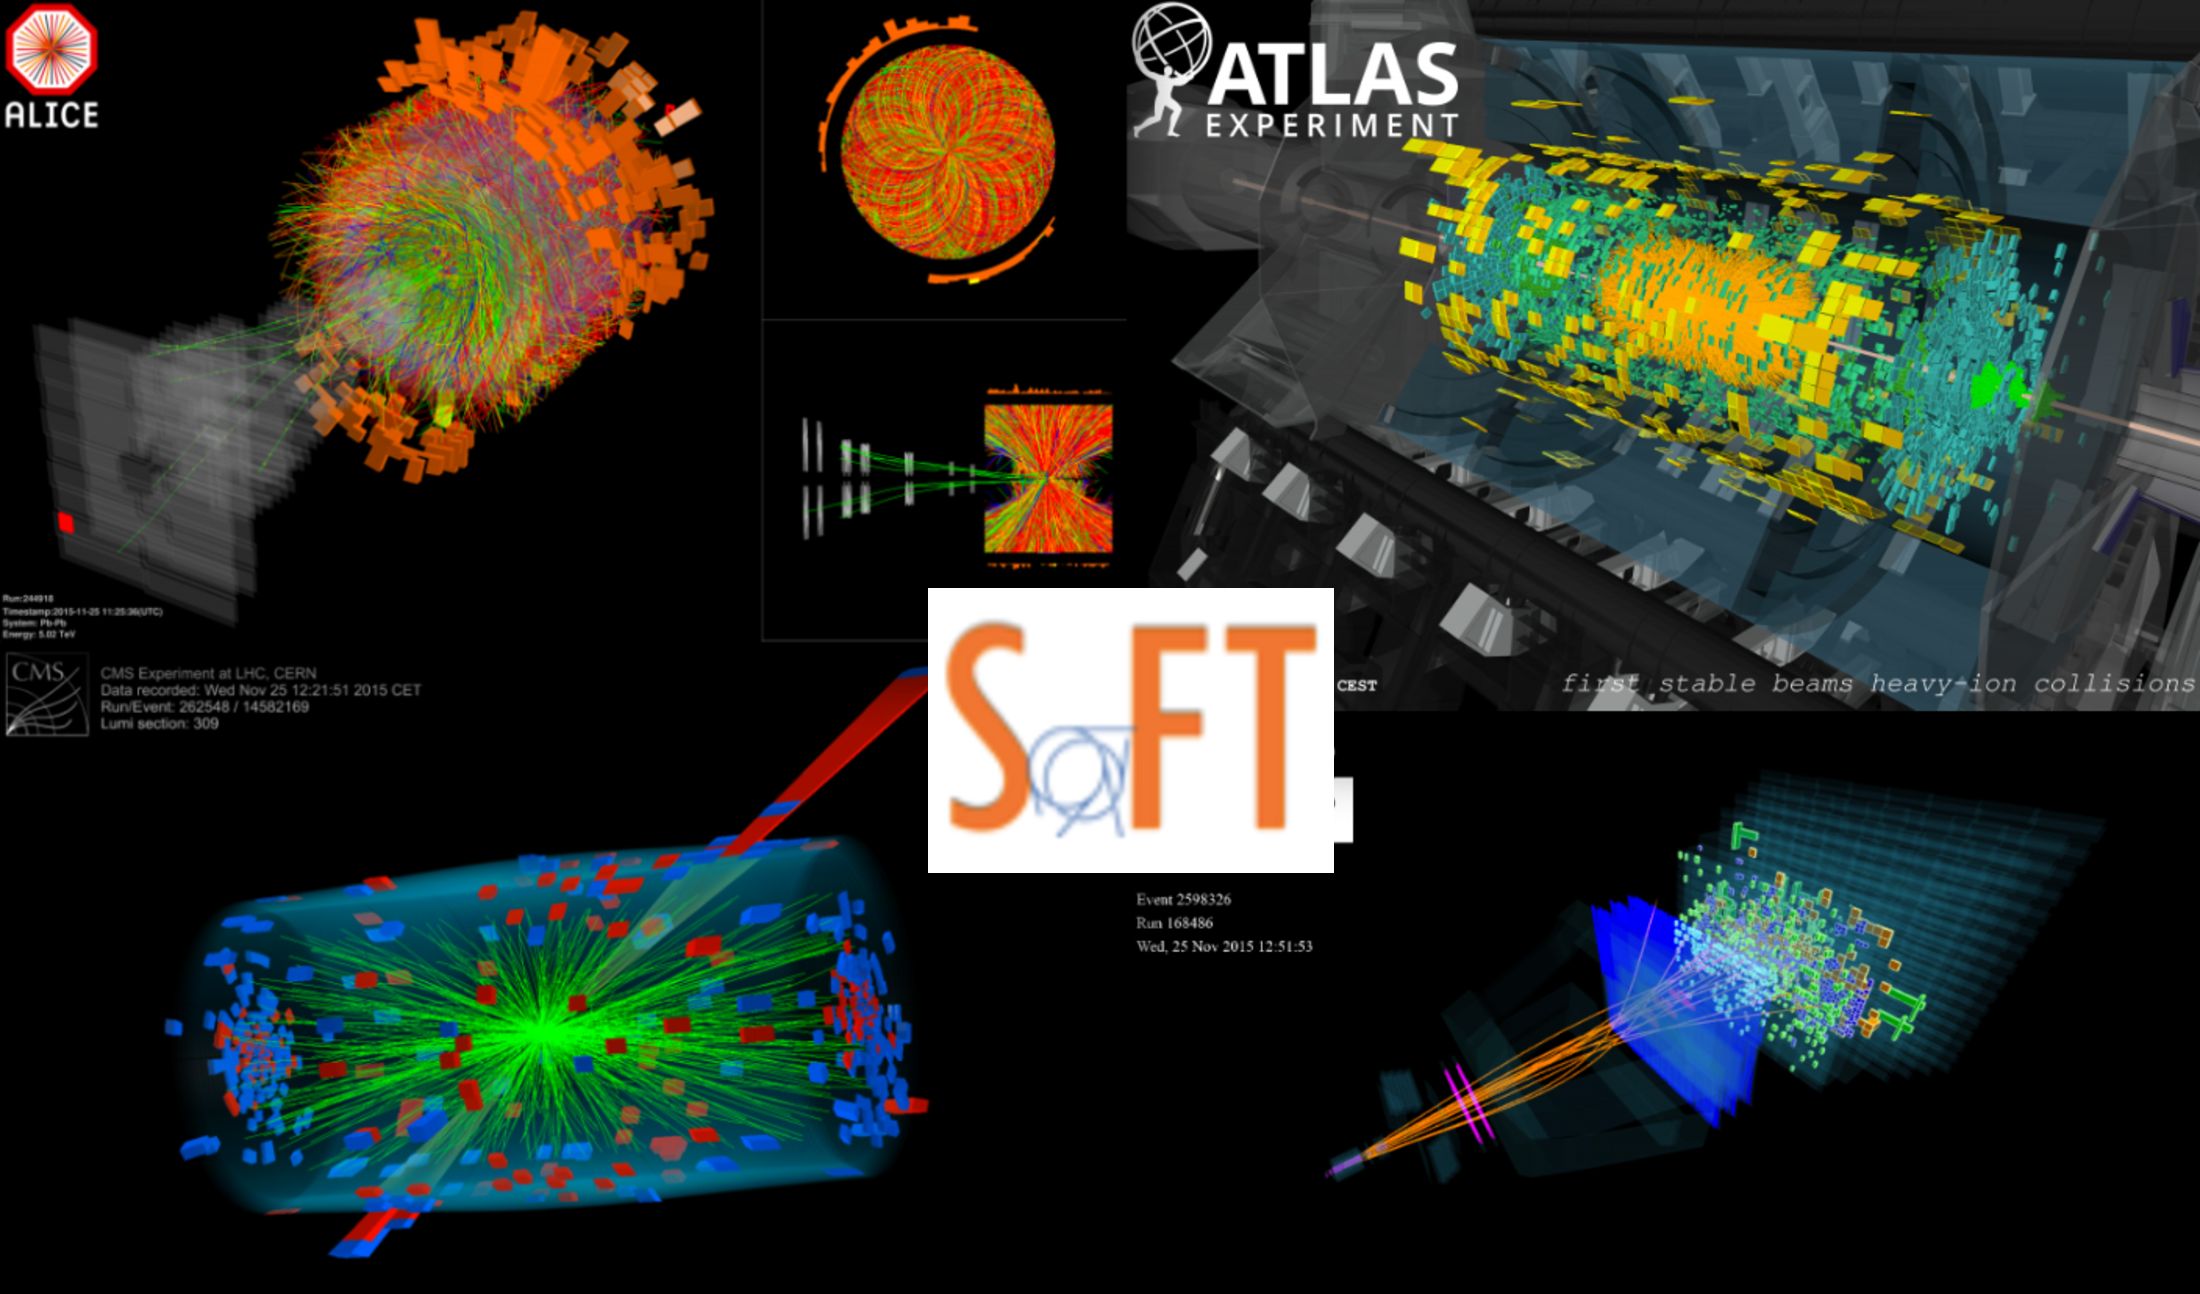
\includegraphics[width=\paperwidth,height=\paperheight]{banner.pdf}%
  }   
  \begin{frame}[t]
    \visible<2>{
      {~}
      \vspace{.5\textheight}
      \begin{columns}
        \begin{column}{.35\textwidth}
        \end{column}
        \begin{column}{.65\textwidth}
          \begin{block}{}
            \IfFileExists{./QR2.png}{
              \footnotesize{slides (excl.\ cern logo) will appear on}

              \gitlablink

              
\includegraphics[width=.2\textwidth]{./QR2.png}
            }{}
          \end{block}
        \end{column}
      \end{columns}
    }
  \end{frame}
  \beamertemplateshadingbackground{Black!03}{White}
